\section{Mechanisms}

As mentioned earlier, we have implemented two backside touch input based mechanisms and a standard soft-QWERTY keyboard. 

\subsection{Backside QWERTY}
This mechanism uses the standard QWERTY layout, but with a few modifications. In this mechanism, the user places his fingers on the backside screen and it results in a cursor appearing on the front screen at a location that is vertically above the touch point. This way user can move multiple cursors at the same time, using multiple fingers. To input a particular character, the user must select a particular key with the cursor and then touch the front screen anywhere to signal input. Figure 3 shows a user selecting a character on the backside-QWERTY mechanism.

\begin{figure}
    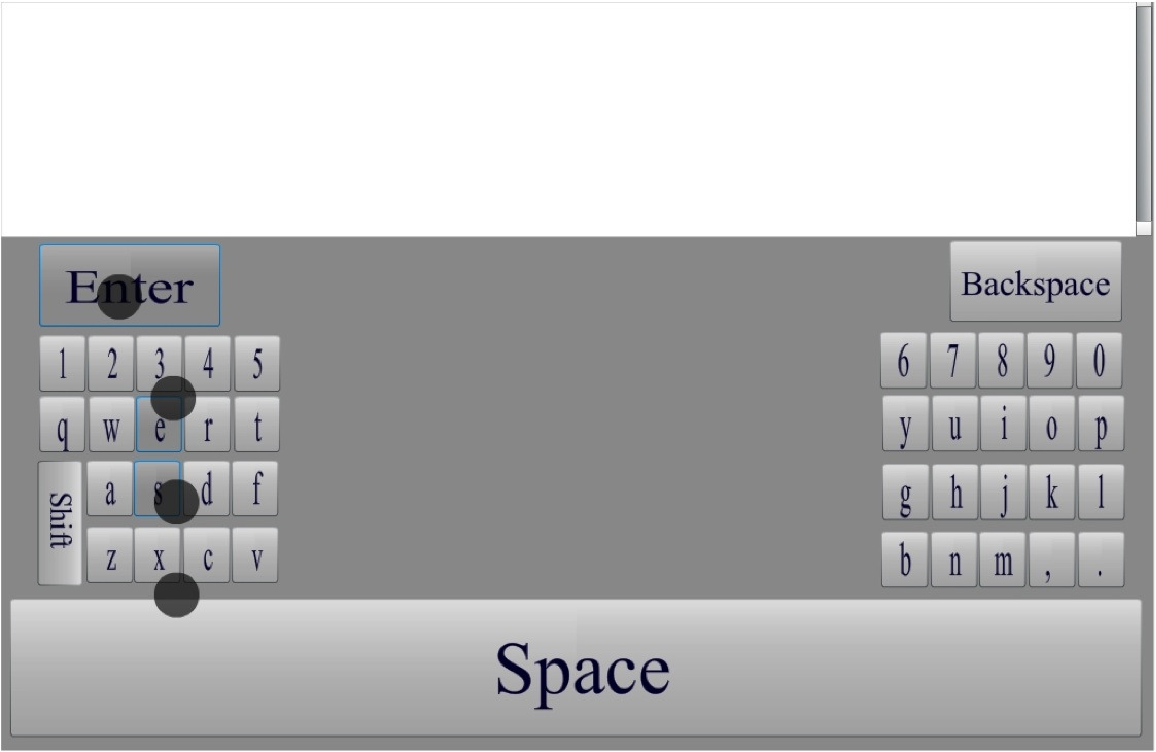
\includegraphics[scale=0.45]{Figures/backside.pdf} 
    \caption{Screenshot of backside-QWERTY with user's fingers on the
      backside screen}
\end{figure}

\subsubsection{Design evolution}

The interface went through two iterations before getting its final shape. The first version used pressure as a method to signal input. When the user increased the pressure on the backside input, a character would be registered.  Unfortunately, pressure input on the Stantum panels appears to be measured by measuring the size of the contact point, rather than actually measuring pressure.  As such, the pressure measurements are inaccurate and difficult to calibrate, especially for the pinky finger. Also, initial tests suggested that being able to control the amount of pressure being applied is hard for users. Since the users were already applying some pressure to drag the cursors around, it turned out to be confusing for them.

Therefore, the second version of the interface accepted a character as input if the user released their finger over that character (also called a "lift-off" at times). However, in this case the chances of giving accidental inputs, by accidentally removing a finger increase manifold. 

As a result we finally shifted to touching (using the thumb) the front panel once the character has been selected, as the method to signal input. This was deliberately done in view of previous research on back-of-device touch input, that advocates the use of thumb-on-front as a complement to fingers on the back techniques. \cite{Wobbrock} 

In the first version we had also modified the keyboard layout to match the finger to key mappings on a QWERTY keyboard, as done by previous research \cite{RearType},\cite{LucidTouch}. However, after the initial test, we realized that users were still doing visual search for keys instead of using their pre-existing motor knowledge of QWERTY. Therefore, a standard QWERTY layout in this case turned out to be more predictable and usable. In hindsight, this is not surprising because previous research \cite{Wobbrock} argued that if finger movement is to be displayed to the user, a "visual-correct" mapping should be used; otherwise a "motor-correct" one may be used. The research on LucidTouch, also indicated that the users were split in terms of their preference for the layout (QWERTY versus inverted-QWERTY). After initial testing, the size of the Space, Backspace and Enter keys was increased to make them easier to select.

\subsection{Chording mechanism}
\begin{figure*}
    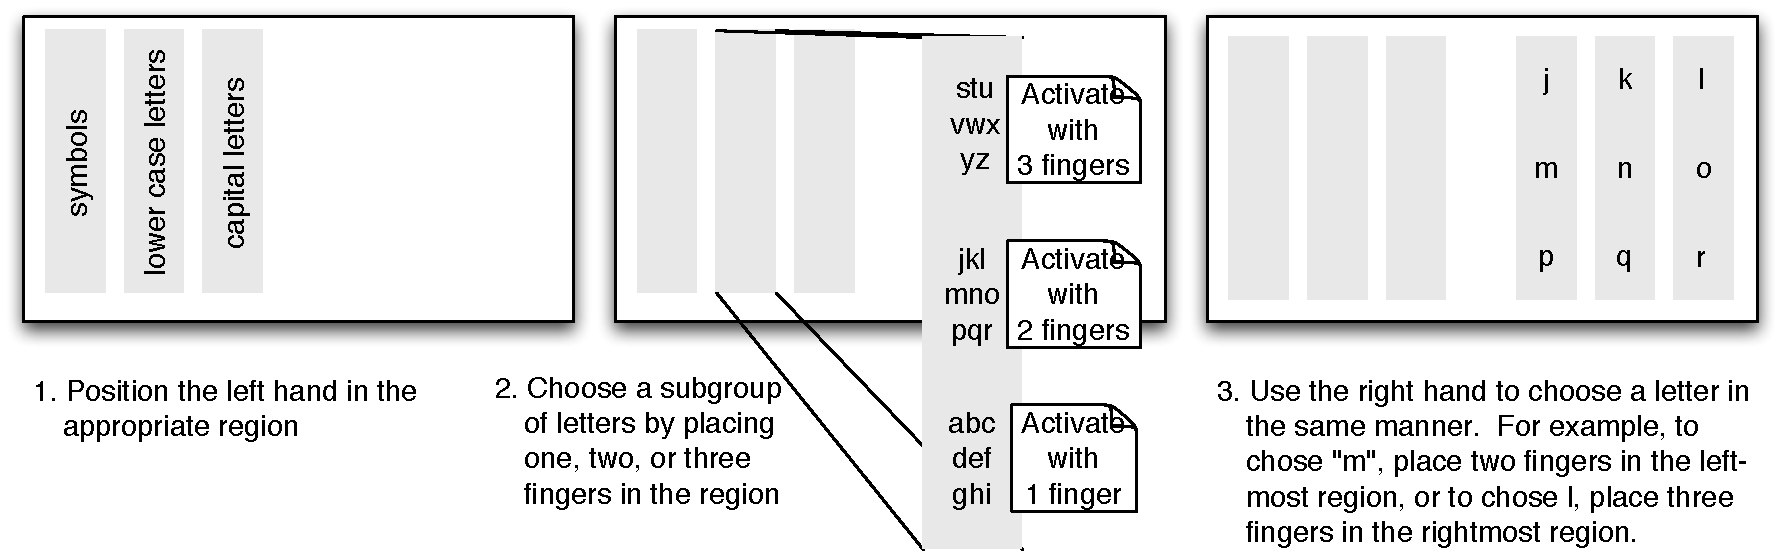
\includegraphics[width=\textwidth]{Figures/chording_explaination.pdf} 
    \caption{Enter the character ``l'' using the chording mechanisms.
      Note that all three steps can be performed simultaneously, for
      proficient users.}
    \label{fig:chording_explanation}
\end{figure*} 

To use the chording mechanism the user extends and contracts their fingers (e.g. move their fingers in the horizontal axis in the natural pose). The user's hand can select three regions, determined exclusively by the distance from the edge of the screen. The movements of the user's left hand select a character class: upper-case, lower-case or symbols. Within these classes, the number of fingers touching the region determines one of three subgroups in the class, with nine characters in each subgroup. The nine characters are broken up into three groups, and the users are supposed to use their right hand to select a character. In summary, the users select a class, a subgroup within a class and a character within the subgroup through each particular configuration of fingers on the back (Figure~\ref{fig:chording_explanation}). It should also be noted that in any given class the user can place one finger to select the lower subgroup, two fingers to select the middle subgroup and three to select the top one.

For example, in Figure~\ref{fig:chording_example} the user places two fingers of the left hand in the middle region to select the class of lower-case letters and the subgroup of "jklmnopqr". The user then places three fingers of the right hand in the rightmost region to select the letter "l".

In our implementation, the number of fingers activating a region is indicated by color changes to the activated regions, in addition to the translucent circles representing the location of the fingers. The user can use these circles to position their fingers in the correct locations. They then touch (using their thumb) anywhere on the front screen to indicate a character input (motivation same as above). Wobbrock et al. \cite{Wobbrock} also talk about the need to minimize vertical movements in back-of-device interactions, which is precisely what our chording mechanism reflects. When the user is learning how to use the chording mechanism, they can enter a character using the step-by-step process described above.  As they become more familiar, however, then can enter chords by touching the device with both hands, in the correct location, simultaneously.

Similar to backside QWERTY and QWERTY, the top quarter of the screen was a scrollable textfield, which displayed the text that was being entered.

The chording mechanism was designed to allow the user to exploit their proprioception (the sense of the relative positions of one's body) rather than tactile feedback, in order to form and exploit kinesthetic memory (short-feedback memory in the nervous system that bypasses cognitive processing for repetitive tasks, often called ``muscle-memory''). Since gross motor movements provide better proprioception, the mechanism was designed to reduce requirements for precise movement.


\begin{figure}
    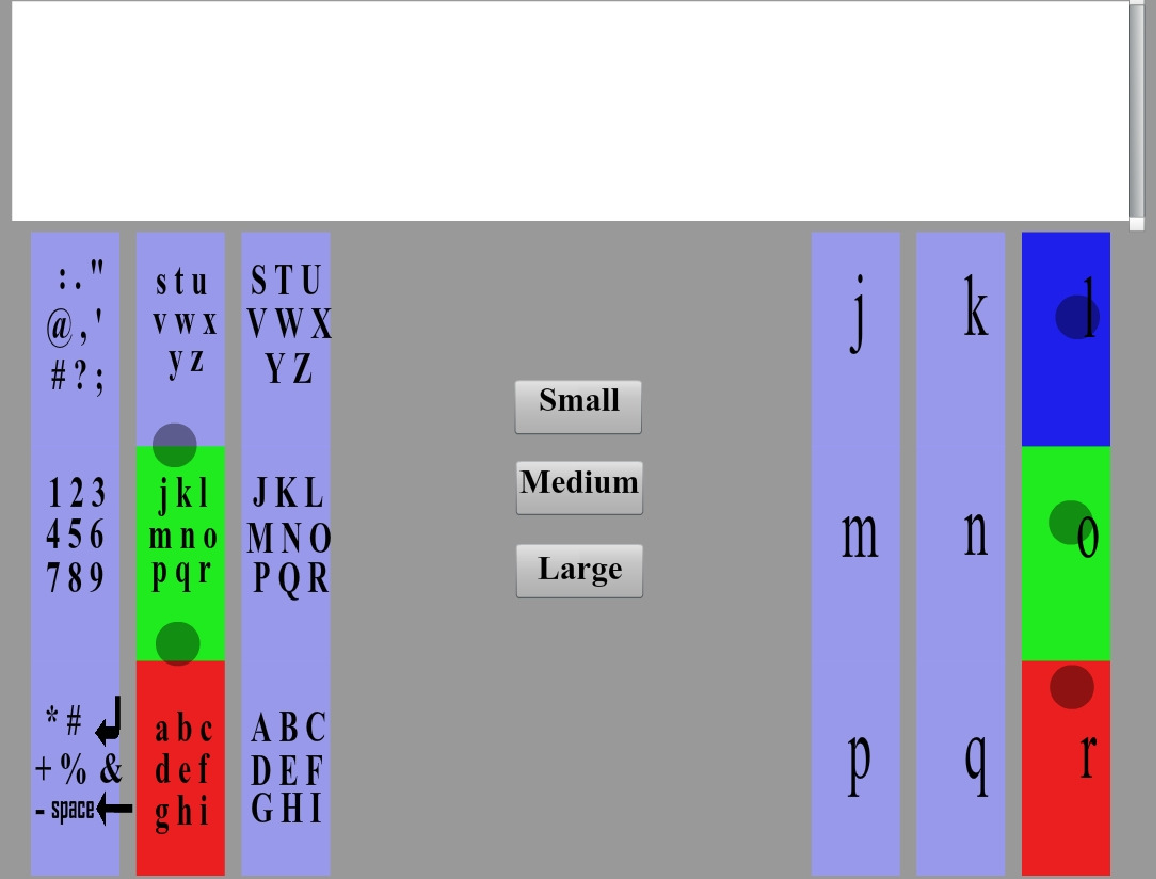
\includegraphics[scale=0.45]{Figures/chording.pdf} 
    \caption{Screenshot of chording mechanism with user's fingers on
      the backside screen trying to form a chord.}
       \label{fig:chording_example}
\end{figure} 
\subsubsection{Design Evolution}

Initial testing suggested that the finger sizes and areas in which users can move comfortably vary a lot. Therefore, in the final version the users were allowed to select from large/medium/small setting, that determined the width of the zones. Users, who had smaller reach, could use these settings to optimize the area of movement. The rest of the design changes pertained to the device itself (like pressure), and therefore the fixes were the same as backside-QWERTY.

\subsection{QWERTY}

This is a standard soft QWERTY keyboard, with no special modifications. The keyboard supports multitouch, which means the users can select the next character to be entered without releasing the currently selected one. The keys turns blue on click, so that the user gets appropriate feedback. The top quarter of the screen is a scrollable textfield, which displays the text that is being entered.
